\chapter{Saturazione}\label{cap:saturazione}

In questa sezione, consideriamo i
calcoli nelle reti ad albero sotto le restrizioni standard \textbf{R} più
chiaramente, la conoscenza comune che la rete è un albero.\\
Si noti che la conoscenza di essere in un albero implica che ogni entità può
determinare se è una \textbf{foglia} (cioè ha un solo vicino) o un nodo interno
(cioè ha più di un vicino).\\
Abbiamo già visto come risolvere i problemi di Broadcast, Wake-Up e Traversal in
una rete ad albero. I primi due sono risolti in modo ottimale dal protocollo
Flooding, il secondo dal protocollo DF Traversal. Queste tecniche costituiscono
il primo insieme di strumenti algoritmici per il calcolo in alberi con più
iniziatori. Introdurremo ora un'altra tecnica molto basilare e utile, la
\textbf{saturazione}, e mostreremo come può essere impiegata per risolvere in
modo efficiente molti problemi diversi negli alberi indipendentemente dal numero
di iniziatori e dalla loro posizione.\\
Prima di farlo, dobbiamo introdurre alcuni concetti e terminologia di base sugli
alberi. In un albero T, la rimozione di un collegamento $(x,y)$
\textbf{disconnetterà T} in due alberi, uno contenente $x$ (ma non $y$), l'altro
contenente $y$ (ma non $x$); li indicheremo rispettivamente con $T[x - y]$ e
$T[y - x]$. Sia $d[x, y]$ = $Max\{d(x, z) : z \in T[y - x]\}$ la distanza
maggiore tra $x$ e i nodi in $T[y - x]$. Ricordiamo che la distanza più lunga
tra due nodi qualsiasi è chiamata \textbf{diametro} ed è indicata con $d$. Se
$d[x, y] = d$, il cammino tra $x$ e $y$ si dice \textbf{diametrale}.

\section{Tecnica di Saturazione}
La tecnica della saturazione consiste nell'avere una configurazione iniziale (al
tempo $t_0$) del nostro sistema in cui tutte le entità sono nello stato di
Asleep (come nel Wake-up) ed avere una configurazione finale in cui il sistema
avrà esattamente due entità nello stato di SATURATED e tutte le altre nello
stato di PROCESSING. Per il funzionamento si assume come grafo un \textbf{albero
    T} non radicato e l'insieme delle restrizioni in cui si lavora è solo \textbf{R,
    si possono avere quindi più iniziatori.} Questa permetterà di trovare
esattamente $2$ nodi vicini tra di loro e la tecnica consiste in tre stadi:

\begin{enumerate}
    \item \textbf{Stadio di attivazione (Wake-Up)}: L'obiettivo è quello di
          eseguire il Wake-up. Viene svolto dagli iniziatori che, una volta diventati
          attivi, mandano un messaggio d'attivazione a tutti i loro vicini che
          diventeranno quindi Active. A loro volta attiveranno i loro vicini. Lo scopo è
          quello di avere tutti i nodi Active (\texttt{Wake-Up}).
    \item \textbf{Stadio di saturazione (Convergecast)}: Viene iniziato dalle
          foglie dello ST. Queste inviano un messaggio $M$ al padre e passano allo stato
          di PROCESSING. Un nodo interno $x$ non appena riceve il messaggio $M$ da
          $deg(x) -1$ vicini, manda $M$ all'unico vicino che non gli ha mandato $M$ e
          considera questo come padre; inoltre passa allo stato di PROCESSING. Infine se
          un nodo nello stato di PROCESSING riceve $M$ da suo padre, passa allo stato di
          SATURATED. Lo scopo è quello di andare ad eleggere due nodi saturi (vedremo
          che sono due).
    \item \textbf{Stadio di risoluzione (Dipende)}: Viene iniziato dai 2 nodi
          saturati e la natura di questo stadio dipende dall'applicazione in cui
          ci troviamo.
\end{enumerate}
Ripetiamo come funziona lo stadio di saturazione:
\begin{itemize}
    \item Una foglia manda un messaggio $M$ al proprio padre.
    \item Un entità non foglia aspetta di ricevere $|N(x)|-1$ messaggi di tipo M.
          Quando questo avviene manda $M$ sull'unico link da cui non lo ha ricevuto.
\end{itemize}
Quindi si avranno: $\#msg(M) = n$, poiché ci sarà un arco in cui transitano due
messaggi, la coppia di nodi di questo arco sarà la \textbf{coppia di nodi
    saturi}, viene infatti definita come tecnica \textbf{Edge-election}, perché è
stato selezionato un arco. Una volta che sono stati
"scoperti" i nodi saturi inizia la fase di Risoluzione, che viene cominciata da
quest'ultimi.

\begin{theorem}
    Esattamente due nodi in stato di PROCESSING diventeranno SATURATED;
    inoltre questi 2 nodi sono l'uno il padre dell'altro (sono vicini).
\end{theorem}
%Per come abbiamo definito l'algoritmo, un'entità invia un messaggio M
%solamente a suo padre, e diventa SATURATED una volta che riceve M da
%quest'ultimo. Prendiamo ad esempio un nodo $x$ che invierà un messaggio M nel
%link che lo collega al suo parent. Prima o poi, dato che non sono presenti
%cicli, il messaggio arriverà ad un nodo SATURATED $s_1$. Questo nodo è
%diventato SATURATED perché ha ricevuto un messaggio M dal suo parent $s_2$;
%poiché s2 ha inviato un messaggio M ad s1, s2 deve essere stato in PROCESSING
%e deve aver considerato s1 suo padre. Quindi quando il messaggio M di s1
%arriverà su s2, anche s2 diventa saturo. Pertanto esistono almeno due nodi
%che diventano saturi.

\begin{proof}[Dimostrazione. \textbf{(Solo due nodi Saturi)} \textit{[Modo 1]}]\
    \begin{figure}[H]
        \centering
        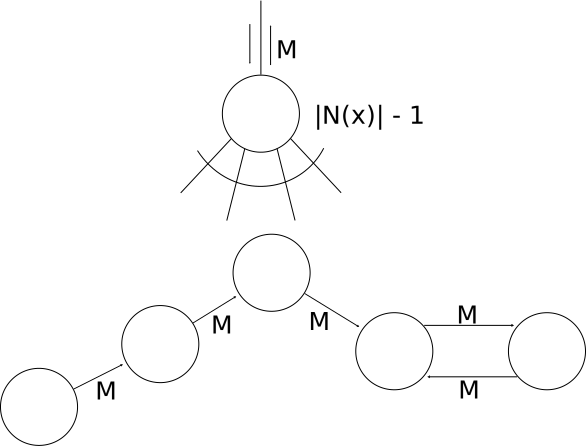
\includegraphics[scale=0.5]{capitoli/saturazione/imgs/n_40}
    \end{figure}

    \textbf{Dimostro che esattamente due nodi diventano Saturated:}
    \begin{enumerate}
        \item Supponiamo che $x$ nodo foglia invia un messaggio $M$ a suo
              padre.
        \item Dato che ci troviamo su un albero non ci saranno cicli, quindi
              prima o poi questo messaggio raggiungerà un nodo $s_1$ in stato di
              SATURATED.
        \item Questo nodo per essere diventato SATURATED deve aver ricevuto
              $M$ da suo padre $s_2$, ma se $s_2$ ha inviato $M$ allora è
              sicuramente in stato di PROCESSING e deve aver considerato
              $s_1$ suo padre.
        \item Quando $M$ inviato da $x$ arriva ad $s_1$, questo lo invia a suo
              padre, che è $s_2$ ma questo è in stato di PROCESSING e riceve $M$,
              quindi diventa SATURATED.
    \end{enumerate}

    %\\ Nel percorso fatto dai messaggi M, prima o poi arriviamo ad un
    %nodo SATURATED poiché siamo in un albero (non abbiamo cicli). In
    %particolare, quando arriviamo al nodo SATURATED, esso invia il
    %messaggio M a suo padre, ma dato che è Saturated allora suo padre è
    %sicuramente in stato di Processing, ovvero ha già inviato un
    %messaggio M. e quindi il nodo prima di lui avrà considerato il
    %messaggio M, 
    Se ne conclude che anche il nodo prima diventa SATURATED. Almeno due
    nodi diventano SATURATED.
\end{proof}

\begin{proof}[Dimostrazione. \textbf{(Solo due nodi Saturi)} \textit{[Modo 2]}]\

    Si può confermare che i nodi
    saturi sono 2 per la correttezza del Convergecast. Durante questo
    protocollo, ogni entità manda esattamente un messaggio, ma dato che le
    entità sono $n$ e gli archi in un albero sono $n-1$, ci sarà per forza
    un arco in cui transiteranno due messaggi $M$, e quell'arco è proprio
    quello che congiunge i due nodi saturi.
\end{proof}
\begin{proof}[Dimostrazione. \textbf{(I nodi Satured sono Vicini)}]\

    Assumiamo, per assurdo, $\exists x,y$ SATURATED con la
    distanza tra di loro maggiore di 2.
    \begin{center}
        $d(x,y) \geq 2$

        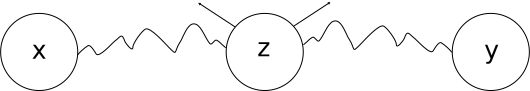
\includegraphics[scale=0.5]{capitoli/saturazione/imgs/n_41}
    \end{center}

    In questo caso affinché $x$ ed $y$ fossero nodi saturi $z$ dovrebbe
    aver mandato due messaggi di tipo $M$, ma questo è assurdo, perché va
    contro le ipotesi del protocollo (non può esistere $z$ che manda due $M$
    nelle due direzioni: ogni nodo manda un solo $M$, questo è assurdo). Se
    ne conclude quindi che i due nodi saturi sono sicuramente vicini tra
    di loro.
    %Non può esistere $z$ che manda due M nelle due direzioni: ogni nodo
    %manda un solo M, questo è assurdo. Contraddice che il nodo centrale
    %dovrebbe inviare due messaggi M, la contraddizione è che tra X ed Y
    %non ci deve essere nessuno se ci fosse, allora quel nodo dovrebbe
    %aver mandato 2 messaggi Min in entrambe le direzioni
\end{proof}

\textbf{Importante:} Quali nodi diventano saturi dipende strettamente dal
ritardo di comunicazione e quindi è totalmente imprevedibile. Esecuzioni
successive con gli stessi iniziatori potrebbero generare coppie di nodi saturi
diverse ad ogni esecuzione.

\subsection{Complessità}
\underline{Messaggi [Prof]:}
$M[$\texttt{SatureTree,R,treee}$] \leq 2(n-1) + (n-1+1) = 3n - 2$
\begin{itemize}
    \item $2(n-1)$ è il costo della prima fase del Wake-Up (con $n$ iniziatori,
          caso peggiore)
    \item $(n-1+1)$ è un singolo messaggio per arco, che in un albero sono $n-1$
          mentre l'unico arco in cui transiteranno due messaggi è quello che
          connette i due nodi saturi, che quindi abbiamo un $+1$.
\end{itemize}
Supponiamo di avere $K^*$ iniziatori:
\begin{center}
    $M[$\texttt{SatureTree,R,tree}$] = n + K^* - 2 + (n-1+1) = 2n + K^* -2$\\
\end{center}
Dove:
\begin{itemize}
    \item $(n + K^* - 2)$ Costo del wake-up con $k^*$ iniziatori.
    \item $(n-1+1)$ uguale a sopra.
\end{itemize}

Durante il processo di saturazione, esattamente un messaggio viene trasmesso su
ogni arco, tranne quello che connette i due nodi saturi, dove $M$ viene inviato
due volte, quindi il totale è $n-1+1 = n$ messaggi.

\underline{Tempo [Prof]:}
$T[$\texttt{SatureTree,R,tree}$] \leq d + d$
\begin{itemize}
    \item Il Primo $d$ è il costo in tempo del Wake-up
    \item Il Secondo è del ConvergeCast (risalita del messaggio dalle foglie)
\end{itemize}
\underline{Tempo:}
Per determinare il tempo ideale siano:
\begin{itemize}
    \item $I \subseteq V$ iniziatori;
    \item $L \subseteq V$ foglie;
    \item $t(x)$ tempo dall'inizio dell'algoritmo fino a che $x$ non diventa
          ACTIVE.
\end{itemize}

Un nodo SATURED $s$ deve aspettare che tutte le foglie siano ACTIVE e che i
messaggi $M$ generati da esse lo raggiungano, quindi deve aver aspettato:
\begin{center}
    $\max \lbrace t(l) + d(l,s) : l \in L \rbrace$
\end{center}

Uno nodo non iniziatore $x$ diventerà ACTIVE al tempo:

\begin{center}
    $t(x) = \min \lbrace d(x,y) : y \in I \rbrace$
\end{center}

Quindi il costo totale è:

\begin{center}
    $T[$\texttt{FullSaturation}$] \leq \max \{ \min \{ d(l,y) \} + d(l,s) : y \in
        I, l \in L \} \leq 2d $
\end{center}

\textbf{ConvergeCast:}
\begin{enumerate}
    \item Una foglia invia un messaggio al parent.
    \item Ogni nodo interno aspetta fin quando non ha ricevuto tutti i messaggi
          dai suoi figli e successivamente invia un messaggio al proprio padre.
\end{enumerate}

\section{Esempio di applicazione: Protocollo MinFind}

$$P_{INIT} = < \forall x \in \xi, value(x) \in \mathbb{R}, status(x) =
    Available>$$
$$
    P_{FINAL} =   <
    \forall x \in \xi, status(x)= MIN \; if \; value(x) = min
    \{value(y), y \in \xi \}$$$$ \wedge status(x) = LARGE \;altrimenti >$$
Vediamo ora un esempio di applicazione della Saturazione per trovare il più
piccolo valore all'interno di un sistema. Ogni entità $x$ ha un certo valore
$v(x)$ ed è in uno stato uguale a tutte le altre (AVAILABLE). L'obiettivo è
quello di trovare il minimo tra tutti i valori $v(x)$ delle entità, e fare in
modo che in terminazione ognuna di esse conosca se è o no il minimo all'interno
del sistema, ed entrare rispettivamente nello stato di MINIMUM o LARGE.\\
\textbf{Attenzione:} L'insieme delle restrizioni sulle quali ci basiamo resta
comunque $R$. Più di un'entità all'interno del sistema può avere il minimo
valore poiché sono ammessi valori uguali tra più entità. Si assume un albero non
radicato come grafo.\\
\begin{itemize}
    \item Se l'albero fosse radicato, allora il problema sarebbe più semplice,
          poiché in questa tipologia, è presente sia un nodo speciale (la radice) sia un
          orientamento logico dei link, infatti ogni nodo può capire quale link è "up",
          ovvero che lo porta alla radice, e quale link è "down", ovvero che lo
          allontana da quest'ultima. In questa tipologia, per trovare il minimo, la
          radice effettua un broadcast di richiesta "down" per richiedere la
          computazione del minimo valore dell'albero. Le entità poi effettueranno quello
          che è il convergecast iniziato dalle foglie. I nodi determineranno il minimo
          valore del proprio sotto albero e lo rispediranno nell'arco "up". Ne risulta
          che il minimo valore è computato alla radice, che effettuerà poi il broadcast
          di questo a tutti. \textbf{Il convergecast} può essere utilizzato solamente in
          un albero RADICATO.
    \item Nel nostro caso però non abbiamo un albero radicato, ma il processo di
          \textbf{Full Saturation} ci permette comunque di risolvere il problema della
          ricerca del minimo. Vediamo come funziona:
\end{itemize}

L'algoritmo inizia sempre con lo stadio di Attivazione, che farà in modo che
tutte le entità siano ACTIVE. A questo punto quando inizia lo stadio di
Saturazione, all'interno del messaggio $M$ che parte dalle foglie, le entità
inseriscono il valore minimo a loro conosciuto, quindi le foglie invieranno
semplicemente il loro \textit{value}, mentre un nodo interno terrà contro del minimo locale
del suo sotto albero ed invierà a suo padre solamente questo. Ne segue che
quando i due nodi saturi saranno eletti, sapranno il valore minimo del proprio
sotto albero, che invieranno in broadcast nello stadio di Risoluzione.
%Nell'algoritmo tutte le entità partono dallo stato di Available (che è lo stesso
%di ASLEEP), tramite impulso spontaneo un'entità inizia la propria esecuzione ed
%invia un messaggio a tutti i suoi vicini per fare in modo che tutte le entità,
%quando inizia lo stadio di Saturazione siano nello stato di ACTIVE. Un nodo
%diventa processing quando manda M al padre. Quando da processing ricevo altri M
%aggiorno il minimo locale.

%\textbf{Funzionamento dell'algoritmo:} Tramite il processo di saturazione
%vengono scambiati i minimi locali di ogni nodo includendo il valore che
%un'entità ha nel messaggio M, fino ad eleggere i due nodi SATURATED che avranno
%ognuno il minimo locale del proprio sotto albero. Questi due nodi si scambiano
%poi i due minimi venendo quindi a conoscenza del minimo globale. A questo punto
%inizia il processo di risoluzione (Stadio 3) dove viene fatto il
%\textbf{Broadcast} del messaggio di minimo su un albero partendo da due radici,
%quindi il costo è il seguente:

\underline{Messaggi:}\\
$M[$\texttt{MinFind,R,tree}$] \leq 3n - 2 + n - 2 = 4n - 4$
\begin{itemize}
    \item $3n - 2$ è il costo della saturazione.
    \item $n$ è il costo del broadcast.
    \item $-2$ sono i messaggi risparmiati sull'arco saturato, dove i nodi già
          conoscono il minimo globale.
\end{itemize}

\begin{center}
    $M[$\texttt{MINFIND,R,tree}$] = n + K^* - 2 + (n-1+1) + (n-2) = 3n + K^* -
        4$\\
\end{center}
Dove:
\begin{itemize}
    \item $(n + K^* - 2)$ Costo del wake-up con $k^*$ iniziatori.
    \item $(n-1+1)$ uguale a sopra.
    \item $n-2$ costo del broadcast che viene avviato dai nodi saturi, risparmiamo
          due messaggi perché i nodi saturi già conoscono il minimo globale.
\end{itemize}
Possiamo vedere che al costo della \textit{FullSaturation}, sono stati aggiunti
$n-2$ messaggi utilizzati nel terzo stadio (\texttt{Broadcast} su albero
partendo da due radici).


\underline{Tempo:}
$T[$\texttt{SatureTree,R,tree}$] \leq 3d$
\begin{itemize}
    \item $d$ nel sottografo del primo nodo saturato
    \item $d$ nel sottografo del secondo nodo saturato
    \item $d$ Broadcast del messaggio
\end{itemize}


Il costo di $T$ ed $M$ è ottimo asintoticamente, poiché è obbligatorio che tutti i
nodi del grafo siano presi in considerazione.\\
\underline{Tempo [Studenti]:}
\begin{center}
    $T[$\texttt{TreeElectMin}$] = T[$\texttt{FullSaturation}$] + \max \{ d(s, x) :
        s \in S, x \in V \} \leq 3d$
\end{center}

Tramite saturazione possiamo risolvere anche: massimo, somma elementi, prodotto,
predicati logici; in pratica tutte le funzioni dette di semigruppo, in cui
valgono le proprietà commutativa e associativa. Si possono fare anche alcune
funzioni statistiche tipo la media. In particolare vedremo di seguito come la
ricerca dell'eccentricità tramite saturazione faccia scendere il costo da $n^2$
a $n$.

\section{Ricerca dell'eccentricità}
La tecnica di base è stata finora utilizzata per risolvere problemi a valore
singolo; cioè problemi la cui soluzione richiede l'identificazione di un unico
valore. Può anche essere utilizzato per risolvere problemi multivalore come il
problema di determinare le \textbf{eccentricità} di tutti i nodi.\\
Utilizziamo adesso la Saturazione per trovare l'eccentricità dei nodi saturi
all'interno dell'albero. Iniziamo con una definizione:\\

\begin{definition}
    L'eccentricità di un nodo $x$, denotata con $r(x)$, è la più grande
    distanza tra $x$ e ogni altro nodo nell'albero: $$r(x) = Max\{d(x,y) : y \in
        V)\}$$ Notiamo che il \textbf{centro} è il nodo con eccentricità minima.
\end{definition}

\begin{definition}
    In un albero, dato un arco $\{x,y\}$ si denota con $T[x - y]$
    l'albero contenente $x$ ma non $y$ ottenuto rimuovendo l'arco $\{x,y\}$
\end{definition}

Applicando la definizione appena descritta si ottengono quindi 2 sottoalberi,
uno che contiene il nodo $x$ che sarà $T[x - y]$, l'altro invece conterrà il
nodo $y$ e sarà $T[y - x]$. \\\\
\textbf{Come si calcola l'eccentricità di un singolo nodo:}\\
Per calcolare la propria eccentricità, un nodo $x$ deve determinare la massima
distanza da tutti gli altri nodi. Per far questo, $x$ deve effettuare il
Broadcasting della richiesta, diventando automaticamente lui la radice
dell'albero, si utilizza poi il convergecast sull'albero radicato in $x$;
facendo questo si colleziona la massima distanza dagli altri nodi.\\
\textbf{Costo messaggi:} $2(n-1)$ dove:
\begin{itemize}
    \item $n-1$ è  per il Broadcast
    \item $n-1$ è per il Convergecast
\end{itemize}
Se volessi utilizzare questo metodo per il calcolo dell'eccentricità di ogni
nodo, si spenderebbe $n(2(n-1))$ poiché ogni nodo effettua un numero di messaggi
pari a $2(n-1)$.\\

\textbf{Il costo per il calcolo dell'eccentricità di ogni nodo con il metodo
    precedentemente descritto è O($n^2$). Mostreremo adesso che tramite la
    saturazione il costo scende a O($n$)}\\

\textbf{Possiamo usare la saturazione per rilevare l'eccentricità di tutti i
    nodi aggiungendo al messaggio $M$ un valore di "altezza".}

\subsection{Calcolo dell'eccentricità di ogni nodo tramite Saturazione: Protocollo Eccentricity}
Il nostro obiettivo è quello di determinare l'eccentricità di ogni nodo. Il
primo passo per la risoluzione del problema consiste nell'applicare la
Saturazione per calcolare l'eccentricità dei due nodi saturi. Da notare che non
sappiamo a propri quali nodi diventeranno saturi, ma basta sapere che quando ci
diventano sapranno sicuramente la loro eccentricità. Per far questo è necessario
includere nel messaggio $M$ inviato da un'entità $x$ al parent $y$ la
\textbf{massima} distanza di $x$ dai nodi del suo sotto albero $T[x-y]$ (che non
contiene y)+ 1, poiché deve arrivare ad $y$. In questo modo un nodo saturo $s$
saprà la distanza $d[s,y]$ per ogni vicino $y$; quindi potrà calcolare la sua
eccentricità. \\
Il nostro obiettivo però è calcolare l'eccentricità di ogni nodo, non solo
quella dei nodi saturi.\\

La cosa interessante è che le informazioni disponibili presso ciascuna entità al
termine della fase di saturazione sono quasi sufficienti per farle calcolare la
propria eccentricità.\\
Consideriamo un'entità $u$; ha inviato il messaggio $M$ al suo genitore $v$,
dopo averne ricevuto uno da tutti gli altri suoi vicini; il messaggio da $y \neq
    v$ conteneva $d[u, y]$. In altre parole, $u$ conosce già la distanza massima da
tutte le entità \textbf{tranne} quelle nell'albero $T[v - u]$. Pertanto, l'unica
informazione che manca a $u$ è $d[u, v] = Max\{d(u, y) : y \in T[v - u]\}$.
Notare che
$$
    d[u, v] = Max\{d(u, y) : y \in T [v - u]\} = 1 + Max\{d[v, z] : z \neq u \in N (v)\}.
$$
Riassumendo, ogni nodo, tranne quelli saturi, \textbf{manca di un'informazione:
    la distanza massima dai nodi dall'altra parte del collegamento che lo collega al
    suo genitore}. Se i genitori possono fornire queste informazioni, l'attività può
essere completata. Sfortunatamente, anche ai genitori mancano le informazioni, a
meno che non siano i nodi saturi.\\
I nodi saturi hanno tutte le informazioni di cui hanno bisogno. Hanno anche le
informazioni che mancano ai loro vicini: sia $s$ un nodo saturo e $x$ sia un
vicino insaturo; a $x$ mancano le informazioni $d[x, s]$; per l'equazione sopra,
questo è esattamente $d[x, s] = 1 + Max\{d[s, z] : x \neq z \in N(s)\}$, e $s$
conosce tutti i $d[s, z]$ (erano inclusi nei messaggi $M$ ricevuti). Quindi, i
nodi saturi $s$ possono fornire le informazioni necessarie ai loro vicini, che
possono quindi calcolare la loro eccentricità. La buona proprietà è che ora
questi vicini hanno le informazioni richieste dai propri vicini (più lontani dai
nodi saturi). Pertanto, la fase di risoluzione di \textit{Full Saturation} può
essere utilizzata per fornire le informazioni mancanti: partendo dai nodi
saturati, una volta che un'entità riceve le informazioni mancanti da un vicino,
calcolerà la sua eccentricità e fornirà le informazioni mancanti a tutti gli
altri suoi vicini.\\

\textbf{ATTENZIONE:} Nello stadio di Risoluzione l'informazione che viene
propagata non è una notifica, poiché è diversa per ogni vicino che la riceve, ma
resta comunque un singolo messaggio.

Gli algoritmi utilizzati nelle tre fasi quindi sono:
\begin{itemize}
    \item Wake-up
    \item Saturazione
    \item Broadcast NON di notifica, ogni entità riceve un informazione diversa.
\end{itemize}
\textbf{Costo dei Messaggi:}
\begin{itemize}
    \item $2n-2$ per il Wake-Up
    \item $n$ per la saturazione
    \item $n-2$ nella fase di risoluzione (Broadcast)
\end{itemize}
Si avranno quindi $4n-4$ messaggi (esattamente come il MinFind).

\textbf{Costo del Tempo:}\\
Paghiamo $d$ per tutte e 3 le fasi, quindi si avrà $3d$.

\section{Calcolo del Centro dell'albero}
Il centro in un grafo/albero è il nodo con eccentricità minore, ovvero il nodo
che ha la distanza minima da ogni altro nodo all'interno del grafo. Da notare
che una rete può avere più di un centro. Risolvere questo problema implica fare
in modo che ogni entità in fase di terminazione entri rispettivamente nello
stato di $center$ o $notCenter$.\\
\subsection{Sviluppo del protocollo}
Per risolvere il problema del Centro possiamo utilizzare il fatto che il centro
è l'entità che ha eccentricità minima. Applicheremo quindi:
\begin{enumerate}
    \item Protocollo Eccentricity per trovare l'eccentricità di ogni nodo. Questa
          parte sarà iniziata dagli iniziatori.
    \item Ultime due fasi del MinFind. Questa parte sarà iniziata dalle foglie che
          tramite il Convergecast potranno inviare M al loro padre che conterrà il loro
          valore di eccentricità.
\end{enumerate}
Infine i saturi invieranno in broadcast il minimo trovato in modo che tutti i
nodi lo conoscano e quindi un'entità può determinare se è centro o meno,
cambiando stato rispettivamente in $center$ oppure $notCenter$.

\textbf{Messaggi:}
\begin{itemize}
    \item $4n - 4$ per l'eccentricity.
    \item $n$ fase risalita della ricerca del minimo (ConvergeCast).
    \item $n-2$ Broadcast finale.
          $$Totale: 6n -6$$
\end{itemize}
\textbf{Tempo:}
\begin{itemize}
    \item $3d$ per Eccentricity.
    \item $d$ per ConvergeCast.
    \item $d$ per il Broadcast.
          $$Totale: 5d$$
\end{itemize}

\subsection{Miglioramento del protocollo di ricerca del Centro}
Possiamo migliorare il protocollo grazie a delle proprietà relative ai centri in
un albero. Siano $d_1[x]$ e $d_2[x]$ il valore più grande ed il secondo valore
più grande tra tutti i valori ricevuti da x durante l'applicazione del
protocollo di ricerca dell'eccentricità, cioè tra la massima distanza tra $x$ ed
i nodi del sotto albero $T[y-x]$ (\textbf{Attenzione: Quindi la massima distanza
    tra $x$ e L'ALTRO sotto albero NON radicato in lui}) per ogni $y$ vicini ad $x$.
In simboli:
\begin{center}
    $d_1[x]$ e $d_2[x]$ sono il valore più grande ed il secondo valore più grande
    in $T[y-x]$
\end{center}
Il centro di un albero ha interessanti proprietà tra le quali:\\

\begin{lemma}
    In un albero o c'è un unico centro o ce ne sono 2 e sono vicini
    tra loro.
\end{lemma}

\begin{proof}
    Supponiamo per assurdo che  esistono due centri $x$ ed $y$ non
    vicini tra loro e sia $p$ il cammino che connette $x$ ad $y$. Visto che abbiamo
    supposto $x$ ed $y$ non vicini allora il cammino $p$ conterrà almeno un altro
    nodo, ma può anche contenere altri sotto alberi radicati in questo nodo.\\
    Il nodo più lontano da $x$ (che quindi ne determina l'eccentricità) può essere:
    \begin{itemize}
        \item o in un sotto albero di $x$: Se così fosse $y$ sarebbe comunque più
              lontano e allora sarebbe solo $x$ il centro.
        \item o in un sotto albero di $y$: Se così fosse $x$ sarebbe comunque più
              lontano e allora sarebbe solo $y$ il centro.
        \item o in un sotto albero di $p$: Se così fosse dovrebbe esistere un centro
              sul Path ma anche questo è assurdo.
    \end{itemize}
    Se ne conclude che non può esistere un cammino tra i due centri.
\end{proof}

\begin{lemma}
    In un albero tutti i centri giacciono su tutti i percorsi diametrali.
\end{lemma}

\begin{lemma}\label{lem:nodo}
    Un nodo $x$ è centro se e solo se $d_1[x]-d_2[x]\leq 1$, inoltre
    se vale la disuguaglianza stretta allora $x$ è l'unico centro.
\end{lemma}

\begin{proof}
    Supponiamo $x$ sia l'unico centro e:
    \begin{itemize}
        \item Se $d_1[x]-d_2[x] > 1$: Se così fosse, il nodo $y$ che determina
              $d_1[x]$ avrebbe distanza minore di $x$ da tutti gli altri e perciò sarebbe
              lui il centro. Ma questo è assurdo perché $x$ è centro per supposizione.
        \item Se $d_1[x]-d_2[x] = 1$: Allora anche il nodo $y$ che determina $d_1[x]$
              sarà un centro perché avrà le stesse distanze di $x$ dagli altri nodi. Ma per
              supposizione $x$ era l'unico centro.
        \item Se $d_1[x]-d_2[x] = 0$: Il lemma vale, perché $x$ è l'unico centro,
              qualunque altro nodo diverso da $x$ andassi a scegliere sarebbe più lontano da
              tutti gli altri nodi.
    \end{itemize}
\end{proof}

\begin{lemma}
    Siano $y$ e $z$ vicini di $x$ tali che $d_1[x] = d[x, y]$ e $d_2 [x] = d[x,
                z]$. Se $d[x, y] - d[x, z] > 1$, allora tutti i centri sono in $T [y - x]$.
\end{lemma}

Il lemma \ref{lem:nodo} ci da le informazioni necessarie per cambiare il protocollo sopra
descritto. Un'entità $x$ può determinare se è o no $centro$ se viene a
conoscenza del valore $d[x,y]$ di ogni suo vicino $y$. Ma questa informazione è
esattamente quella che viene data ad un entità dall'applicazione del protocollo
Eccentricity. Questo comporta che per risolvere il problema del centro è
necessario solamente il suddetto protocollo. Quando un'entità ha l'informazione
necessaria a computare il suo raggio, controllerà se il più grande valore ed il
secondo più grande valore che ha ricevuto differiscono di almeno uno. Se così
fosse allora diventerà $centro$, altrimenti cambierà stato in $notCenter$

\paragraph{Calcolo del Costo:}
nel protocollo precedentemente descritto si utilizza solamente l'Eccentricity e
qualche calcolo addizionale, ma comunque il costo resta il medesimo di
quest'ultimo protocollo.
\begin{itemize}
    \item Messaggi: $4n - 4$
    \item Tempo: $3d$
\end{itemize}
